\chapter{Implementazione}
\label{implementazione}

\section{Modalità di computazione}
\label{computationMode}
\subsection{Low Computation mode}

\subsection{High Computation mode}

\subsection{Testing Computation mode}
\label{tcm}


\section{Canali di comunicazione}

\subsection{I2C}
\label{imp_i2c}
Per la comunicazione tra l' \textbf{IMU} e il \textbf{Microcontrollore}, si è utilizzato un canale di comunicazione seriale bifilare noto come \textit{Inter Integrated Circuit}, abbreviato \textbf{I2C}.\\
Il protocollo \cite{i2cWiki} dell'I2C richiede due linee seriali per comunicare correttamente:
\begin{itemize}
\item SDA (\textit{Serial Data}) per i dati
\item SCL (\textit{Serial Clock}) per sincronizzare i dispositivi
\end{itemize}
Vanno inoltre aggiunte una connessione di riferimento alla massa e una alla linea di alimentazione (tipicamente 5 o 3,3 V) a cui sono connessi resistori di \textit{pull-up}, come mostrato dalla figura seguente:
\begin{figure}[H]  
	\centering 
	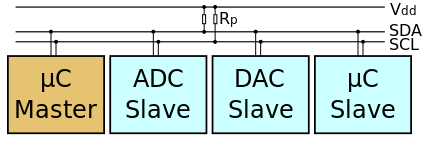
\includegraphics[scale=0.6]{implementazione/i2c.png}
	\caption{Rappresentazione di dispositivi collegati mediante I2C}
	\label{fig:i2c}
\end{figure}
L'I2C utilizza un indirizzo a 7 bit per un totale di 128 indirizzi disponibili. Poiché di questi 16 sono riservati, si ha un totale finale di 112 dispositivi collegabili alla medesima linea.\\
La velocità è il grande limite di questa comunicazione, infatti con le recenti revisioni si è riuscita a raggiungere una velocità massima di 3,4 Mbit/s (detto anche \textit{High Speed Mode}). Nello specifico di questa tesi lo si è utilizzato in \textit{fast mode} che corrisponde ad una velocità di 400 Kbit/s.\\
I dispositivi collegati al bus possono essere di due tipi:
\begin{itemize}
\item Un \textit{Master} che controlla la SCL, inizializza le comunicazioni e invia dati
\item Uno o più \textit{Slave} che rispondono ad un master e inviano dati
\end{itemize}

Il messaggio viene spezzato in due parti:
	\begin{itemize}
		\item \textit{Address frame} dove il \textit{master} indica l'indirizzo dello \textit{slave} interessato alla comunicazione
		\item uno o più \textit{Data frames} contenenti l'informazione da trasmettere
	\end{itemize}
I dati sono "piazzati" sulla linea SDA dopo che la linea SCL è posta a zero dal master, questi dati verranno letti dal dispositivo specificato nell'\textit{address frame} quando il \textit{master} riporterà la linea SCL al valore alto.\\
Relativamente al lavoro di questa tesi si identificano il \textit{Microcontrollore} come \textit{master} mentre l'\textit{IMU} come \textit{slave}. Nello specifico la comunicazione consiste nella lettura periodica da parte del microcontrollore dei valori misurati dai sensori all'interno dell'IMU. Tale lettura è stata realizzata leggendo i singoli registri ad 8 bit dei sensori (per maggiori dettagli si veda la stima temporale in sez.\ref{analisiTemporale}) attraverso lo script in Appendice \ref{scriptXLGRead} e rappresentato dalla seguente figura:
\begin{figure}[H]  
	\centering 
	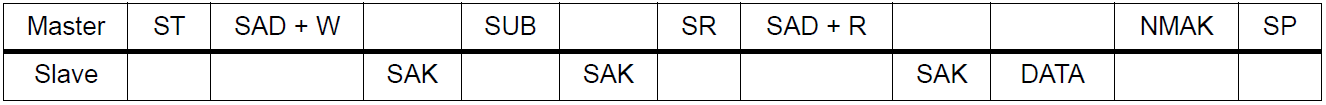
\includegraphics[scale=0.5]{implementazione/i2cRead.png}
	\caption{Rappresentazione del flusso di dati generato per la lettura, tramite I2C, di un registro ad 8 bit.}
	\label{fig:i2cRead}
\end{figure}
 Dove:
 \begin{itemize}
	\item  \textit{ST} è il segnale di inizio di una comunicazione
	\item \textit{SAD + W} include l'indirizzo del dispositivo slave mentre l'ultimo bit specifica che il master sta per scrivere
	\item \textit{SAK} lo slave con l'indirizzo specificato precedentemente risponde con un segnale di \textit{acknowledge}
	\item \textit{SUB} è l'indirizzo del registro interno del dispositivo specificato precedentemente
	\item \textit{SAK} lo slave risponde con un segnali di \textit{acknowledge} se l'indirizzo del registro esiste
	\item \textit{SR} è il bit di ripetizione dello start utilizzato in combinazione con SAD+R/W
	\item \textit{SAD + R} include l'indirizzo del dispositivo slave mentre l'ultimo bit specifica che il master vuole ricevere dati
	\item \textit{SAK} segnale di \textit{acknowledge} da parte dello \textit{slave}
	\item \textit{DATA} dati trasmetti nel formato ad 8 bit
	\item \textit{NMAK} segnale di  \textit{non acknowledge} da parte del \textit{master}
	\item \textit{SP} bit di stop della comunicazione
\end{itemize}
Tuttavia questa lettura non è sempre la migliore, infatti è possibile continuare a leggere i registri interni dello \textit{slave} trasmettendo il segnale di \textit{MAK} invece del segnale di \textit{NMAK} mostrato in Fig.\ref{fig:i2cRead}. In questo modo l'IMU incrementerà l'indirizzo del registro interno di partenza specificato in \textit{SUB} e provvederà a trasmettere il valore del registro interno successivo ad esso. Questa funzionalità è molto utile quando si devono leggere dati, come in questo caso, che sono rappresentati con più registri. Così facendo infatti si riduce l'\textit{overhead} della trasmissione e si migliora quindi il goodput generale rispetto alla lettura ripetuta dei singoli registri.
 
	
\subsection{USB CDC}
\label{imp_usbcdc}